\documentclass[conference,a4paper]{IEEEtran}
\usepackage[T1]{fontenc}
\usepackage[utf8]{inputenc}
\usepackage{amsmath,amssymb}
\usepackage{graphicx,booktabs,cite,url}
\usepackage[hidelinks]{hyperref}
\urlstyle{same}
\hypersetup{pdftitle={B4T: Possession from Incomplete Football Tracking},
 pdfauthor={Marco Giamberduca; Adrian Castano; Ariel Alvano},
 pdfsubject={RAG Phinha -- More Than A Hack 2027 Initial Challenge}}
\title{B4T: Possession from Incomplete Football Tracking}
\author{\IEEEauthorblockN{Marco Giamberduca, Adri\'an Casta\~no and Ariel Alvano}
\IEEEauthorblockA{RAG\_Phinha\\More Than A Hack 2027 -- Initial Challenge}}
\begin{document}
\maketitle
\pagestyle{plain}
\raggedbottom
\begin{abstract}
B4T estimates possession from incomplete automatic football tracking. It first
combines ball observations with team movement, then decodes one home, away or
dead-ball label per frame. Four recurrent components, three seeds and team-swap
averaging provide the frame evidence. Training uses external provider-labelled
matches and simulated tracking errors. The selected two-second recipe reaches
development spellF1 of 0.7309 against a two-second DFL reference, 0.7376 against
a three-second reference, and 0.6829 on SkillCorner. We describe the label
construction, reference-dependent trade-off and commands for exact CPU
regeneration.
\end{abstract}
\begin{IEEEkeywords}
football analytics, possession, tracking data, sequence modelling
\end{IEEEkeywords}

\section{Task and design}
For each of the 199,319 BAR-ATH frames, the challenge asks for home possession
(H), away possession (A), dead ball (D), or X outside the scored
periods~\cite{challenge}. Ranking uses spellF1, which matches H/A possession
intervals of the same team one-to-one by temporal intersection over union: overlapping duration
divided by total covered duration. F1 is averaged over thresholds 0.3, 0.4, 0.5,
0.6 and 0.7. D intervals are not scored as possession objects, so these results
do not separately measure dead-ball detection.

The tracking is automatic and uncorrected. The official documentation reports
that the ball is missing in about 41\% of graded frames. We therefore use both
teams' shape and movement as well as the ball. The method has two steps:
estimate frame evidence, then choose a coherent sequence for each half
(Fig.~\ref{fig:pipeline}).

The selected pipeline reads tactical tracking and match metadata. Video,
homography and Smart Tagging are not inputs. It applies no fixed dead-ball
interval or manual output correction.

\begin{figure*}[t]
\centering
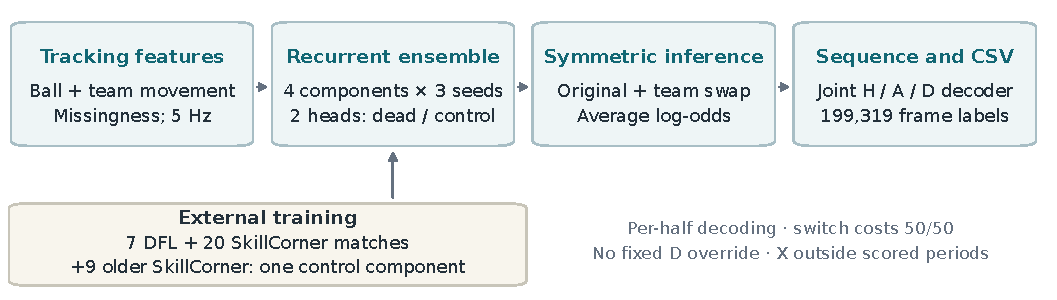
\includegraphics[width=\textwidth]{figures/pipeline.pdf}
\caption{From tracking to possession labels. External matches train the 24
binary recurrent heads; challenge inference uses tracking and metadata. Team-swap
predictions are mapped back before averaging. Fixed dead-ball cues enter the
joint decoder.}
\label{fig:pipeline}
\end{figure*}

\section{External data and reference labels}
Table~\ref{tab:data} lists the labelled sources. We construct external references
from provider metadata:
\begin{itemize}
\item \textbf{DFL:} BallStatus supplies live/dead status and BallPossession supplies
the team.
\item \textbf{Current SkillCorner:} H/A follows the team in each possession phase.
Within a period, the complement of those phases becomes D; outside the periods
it is X.
\item \textbf{Older SkillCorner:} per-frame team possession supervises only the
control head of one component. Unknown possession does not supervise D.
\end{itemize}
DFL uses TRACAB positions; SkillCorner estimates tracking from broadcast video.
The releases differ in coverage and label meaning.

\begin{table}[t]
\caption{External training sources. Match counts are distinct within each release;
training copies do not add independent matches.}
\label{tab:data}
\centering\small
\begin{tabular}{@{}p{0.31\columnwidth}rp{0.43\columnwidth}@{}}
\toprule
Source & Matches & Labels and role \\
\midrule
{\raggedright Sportec/DFL~\cite{bassek2025}\par} & 7 & {\raggedright Ball status and team possession; both heads\par} \\
{\raggedright SkillCorner~\cite{skillcorner}\par} & 20 & {\raggedright H/A phases; D from phase complement; both heads\par} \\
{\raggedright SkillCorner 2019/20~\cite{skillcornerlegacy}\par} & 9 & {\raggedright Per-frame possession; team head in one component\par} \\
\bottomrule
\end{tabular}
\end{table}

For DFL and older SkillCorner, an H/A run shorter than two seconds is reassigned
to the preceding team within the same live segment. D and X reset that process.
This training-reference convention approximates the difference between a touch
and controlled possession (Fig.~\ref{fig:reference}). Current SkillCorner phases
keep their provider H/A labels.

Training simulates long ball gaps, player dropout and coordinate noise. The
base scenario, \texttt{combined\_dead}, also removes the ball with probability
0.8 within each dead-ball interval. Additional copies vary the gap pattern and
random seed; team swapping rotates the pitch and exchanges H/A. Every copy of a
held-out match stays outside all components' training partitions, including
fitted preprocessing.

The repository records fixed versions and file identities. DFL is CC BY 4.0;
both SkillCorner releases are MIT-licensed. Challenge assets are supplied
separately.

\section{Method}
\subsection{Step 1: estimate frame evidence}
Each component has two separate binary bidirectional gated recurrent unit
(BiGRU) models~\cite{cho2014}: dead-ball probability and home-control probability
during live play. They read 5 Hz features in 60-second windows within each half.

Features describe shape, attacking direction, forward movement, pressure,
player speed and observation coverage; the control model also uses the ball.
Missing values become zero with a missingness indicator. Normalisation is
fitted on training frames. Each model uses two recurrent layers, 64 hidden
units per direction and dropout 0.2. Training uses AdamW, 4,000 steps, batch size
64, maximum learning rate $10^{-3}$ and weight decay $10^{-4}$.

The four components are a base recipe; that recipe with extra degraded DFL
copies; a variant with older SkillCorner control supervision; and an audit
variant with an additional dead-ball-missing copy, revised ball-speed features and
window averaging. Three seeds and two heads per component give 24 weights.
Overlapping-window predictions are averaged and interpolated to input frames.

We also predict a view with teams exchanged and the pitch rotated. After
mapping it back to the original team identities, we average views, seeds and
components with equal weight in log-odds space.

\subsection{Step 2: decode the sequence}
Let $c_t$ be signed team-control evidence and $d_t$ dead-ball evidence.
The latter combines the learned model with fixed cues for ball-out, collective
stillness and fast ball movement. A missing ball contributes only together
with stillness. State scores are
\begin{equation}
s_t(H)=c_t-d_t,\quad s_t(A)=-c_t-d_t,\quad s_t(D)=d_t+|c_t|.
\end{equation}
Viterbi decoding chooses the best H/A/D sequence for each half:
\begin{equation}
\underset{\mathbf z\in\{H,A,D\}^{T}}{\arg\max}
\left[\sum_t s_t(z_t)-\sum_{t>1}\lambda(z_{t-1},z_t)\right].
\end{equation}
Changing team costs 50; entering or leaving D costs 50; staying in the same
state costs zero. D$\rightarrow$H and D$\rightarrow$A have equal cost, so a
stoppage resets ownership. The implementation reference gives cue weights,
interpolation and tie handling.

\subsection{Possession conventions}
Loose balls and challenges have no separate class. The sequence keeps the team
supported by the observations until switching is preferred. A restart is a
transition from D to H or A; restart types and individual ball carriers are not
classified. X is written outside the scored periods.

\begin{figure}[t]
\centering
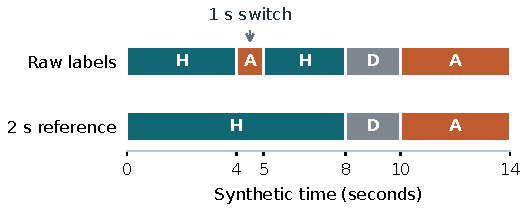
\includegraphics[width=\columnwidth]{figures/training_reference.pdf}
\caption{Synthetic example of the two-second training reference. The one-second
A run is absorbed into H; D separates the later A possession. This transforms
external reference labels, rather than imposing a hard two-second minimum on
the decoded predictions.}
\label{fig:reference}
\end{figure}

\section{External development evidence}
DFL evaluation holds out each of seven matches in turn. SkillCorner uses four
grouped folds over 20 matches. We use the unmodified official scorer and report
match-mean spellF1. Raw denotes the supplied DFL BallPossession flag.
The training threshold and evaluation reference are separate choices.

Clean keeps the external tracking as received. Degraded applies the training
degradation to the held-out match too, using external D labels to remove the ball
with probability 0.8 per interval. The predictor receives only corrupted
observations. The 40\% gaps condition removes ball observations
in 2--30 second gaps, targeting 40\% of each period. These synthetic conditions
do not establish equivalence to the challenge's missingness pattern.

\begin{table}[t]
\caption{Development spellF1 for separately trained recipes. DFL rows are match means ($n=7$); SkillCorner uses provider phases ($n=20$). $\Delta$ is two-second minus three-second training.}
\label{tab:results}
\centering\footnotesize
\begin{tabular}{@{}llrrr@{}}
\toprule
Input & Reference & 3 s & 2 s & $\Delta$ \\
\midrule
Degraded & Raw & 0.5250 & \textbf{0.5607} & +0.0357 \\
 & 2 s & 0.7015 & \textbf{0.7309} & +0.0293 \\
 & 3 s & \textbf{0.7407} & 0.7376 & $-0.0031$ \\
\midrule
Clean & Raw & 0.5348 & \textbf{0.5854} & +0.0506 \\
 & 2 s & 0.7106 & \textbf{0.7426} & +0.0320 \\
 & 3 s & \textbf{0.7528} & 0.7346 & $-0.0183$ \\
\midrule
40\% gaps & Raw & 0.5132 & \textbf{0.5574} & +0.0442 \\
 & 2 s & 0.6816 & \textbf{0.7145} & +0.0329 \\
 & 3 s & \textbf{0.7270} & 0.7121 & $-0.0149$ \\
\midrule
SkillCorner & Phases & 0.6791 & \textbf{0.6829} & +0.0038 \\
\bottomrule
\end{tabular}
\end{table}

\begin{figure}[t]
\centering
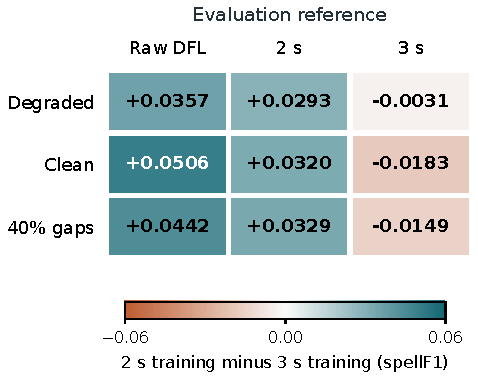
\includegraphics[width=\columnwidth]{figures/reference_tradeoff.pdf}
\caption{Where two-second training gains and loses on DFL. Each cell is the
difference between match-mean spellF1 values for the two recipes, under the same
input and reference ($n=7$). Signed values and a zero-centred scale preserve
both directions of the trade-off.}
\label{fig:tradeoff}
\end{figure}

\noindent\begin{minipage}{\columnwidth}
Table~\ref{tab:results} and Fig.~\ref{fig:tradeoff} compare the recipes.
Against the two-second reference, mean DFL gains are 0.0293--0.0329, with
seven wins in seven matches for each input. Against three seconds, losses
are 0.0031--0.0183. SkillCorner gains 0.0038. These gains favour two-second training.
\end{minipage}

\newpage
\subsection{Development record}
Training and decoder comparisons used external matches. Published challenge
baseline scores informed the original degradation and three-second reference.
The published sensitivity table, derived from ground truth, partly motivated
finer-reference trials. The selected recipe retains the degradation.
The repository's Sources document records the development history.
Costs 50/50 were retained post hoc although E15's registered rule selected
12.5/12.5. Input-only E16 did not select the scenario or change the candidate.
There is no untouched external test set.

\section{Limitations and next steps}
Team-control errors remain the main weakness. Few independent training matches,
different provider labels and camera shift limit transfer. Simulated errors
cover only part of the tracking problems. The two-second transformation is a
working definition of control, and the reference-dependent scores show its
consequences; they do not estimate the private-match score.

We explored hand rules, visibility gating, a second prediction layer, extra
seeds, higher sampling, pseudo-labels and learned switch costs. They did not
replace the selected method. Next, we would improve ball-carrier evidence and
test on another provider.

\section{Reproduction}
The repository includes the card, all 24 weights, pinned dependencies and
training/inference code. Use Python 3.11 and the unmodified official reader at
commit \texttt{f8f2629}. From a Git checkout, follow the README's PowerShell or
Bash commands with the authorised data path and a new run name.

{\raggedright
The commands use the virtual-environment interpreter and check repository integrity.
They run \texttt{scripts/predict\_final.py} with these arguments:
\begin{itemize}
\item \texttt{-{}-model}: \texttt{models/casti-ens4-joint-tta-c2}.
\item \texttt{-{}-data-dir} and a new \texttt{-{}-name}.
\item \texttt{-{}-check-repeat} and the full \texttt{-{}-expected-sha256}.
\end{itemize}
They then validate the CSV. A failed check stops the process.\par}

The expected hash, identical repeat bytes and official validation were obtained
in three Windows environments: an existing Python 3.11.1 installation with
NumPy 1.26.4, PyTorch 2.5.1+cpu, scikit-learn 1.8.0 and one thread (900.9 seconds
for two predictions); a fresh Python 3.11.9 installation following the README;
and Python 3.11.9 with PyTorch 2.5.1+cu124 on CPU, one thread. The third used a
development branch with Smart Tagging but matched the unmasked candidate.

Casti also reported the same checks from a fresh Debian Docker installation
(Python 3.11.18, PyTorch 2.5.1+cpu, one thread). These runs preceded the early
checkout check added to the wrapper; the prediction functions and weight bytes
are unchanged.
The team-named output is \texttt{RAG\_Phinha.csv}. Code and weights have separate
Apache 2.0 declarations. The repository preserves source licences and attribution.

\begin{thebibliography}{6}
\bibitem{challenge}
Metrica Sports, FC Barcelona, and Mobile World Capital Barcelona,
\emph{More Than A Hack 2027: Initial Challenge}, 2026, commit
\texttt{f8f2629}.
[Online]. Available: \url{https://github.com/metrica-sports/more-than-a-hack-2027}
\bibitem{bassek2025}
M. Bassek, R. Rein, H. Weber, and D. Memmert,
\emph{An integrated dataset of spatiotemporal and event data in elite soccer},
Scientific Data, vol. 12, art. 195, 2025,
doi: \href{https://doi.org/10.1038/s41597-025-04505-y}{10.1038/s41597-025-04505-y}.
Dataset: figshare v1, doi:
\href{https://doi.org/10.6084/m9.figshare.28196177.v1}{10.6084/m9.figshare.28196177.v1}.
\bibitem{skillcorner}
SkillCorner, \emph{Open Data}, commit
\texttt{4340d274}.
[Online]. Available: \url{https://github.com/SkillCorner/opendata}
\bibitem{skillcornerlegacy}
SkillCorner, \emph{Open Data, 2019/20 release}, commit
\texttt{1ed50b7}.
[Online]. Available: \url{https://github.com/SkillCorner/opendata}
\bibitem{cho2014}
K. Cho \emph{et al.}, \emph{Learning phrase representations using RNN
encoder--decoder for statistical machine translation}, in Proc. EMNLP,
2014, pp. 1724--1734, doi:
\href{https://doi.org/10.3115/v1/D14-1179}{10.3115/v1/D14-1179}.
\end{thebibliography}
\end{document}

